\documentclass[sigconf]{acmart}

\usepackage[T1]{fontenc}
\usepackage{lmodern}
\usepackage{graphicx}
\usepackage{amsmath}
\usepackage{amssymb}
\usepackage{booktabs}
\usepackage{url}
\usepackage{xcolor}
\usepackage{tikz}
\usepackage[ruled,vlined,linesnumbered]{algorithm2e}
\usetikzlibrary{arrows.meta, positioning, shapes.geometric, fit, backgrounds, calc}
\microtypesetup{expansion=false}

\setcopyright{none}
\acmConference[DAI 2026]{The 8th International Conference on Distributed Artificial Intelligence}{Nov 29--Dec 2, 2026}{Hong Kong, China}

\begin{CCSXML}
<ccs2012>
<concept>
<concept_id>10010147.10010178.10010187</concept_id>
<concept_desc>Computing methodologies~Multi-agent systems</concept_desc>
<concept_significance>500</concept_significance>
</concept>
<concept>
<concept_id>10010147.10010257.10010293.10010294</concept_id>
<concept_desc>Computing methodologies~Cooperation and coordination</concept_desc>
<concept_significance>500</concept_significance>
</concept>
</ccs2012>
\end{CCSXML}

\ccsdesc[500]{Computing methodologies~Multi-agent systems}
\ccsdesc[500]{Computing methodologies~Cooperation and coordination}

\begin{document}

\title{From Topics to Factors: Multi-Agent Verification with Deliberative Consensus}

\author{Anonymous Authors}
\affiliation{%
  \institution{Anonymous Institution}
  \city{Anonymous City}
  \country{China}
}
\email{anonymous@anonymous.com}

\begin{abstract}
LLM-driven factor discovery pipelines transform user-provided investment topics into executable trading factors through multiple generation stages. A critical challenge is error propagation: hallucinated relations or incoherent hypotheses at early stages contaminate downstream factor expressions and portfolio decisions. We address this through a \textbf{multi-agent verification architecture} that deploys independent scorer LLMs at each semantic transition (entity $\rightarrow$ relation $\rightarrow$ hypothesis $\rightarrow$ factor). A key design question is how to fuse scores from multiple scorers. We show that simple averaging---the default in most multi-LLM systems---degrades accuracy in 55\% of disagreement cases (bootstrap 95\% CI: 46--63\%, $n{=}130$ across 6 model pairs), because it gives equal weight to correct and incorrect scorers. Our solution is a \textbf{deliberative consensus protocol}: when scorers disagree beyond a threshold, they enter structured multi-turn debate where they exchange reasoning traces and independently re-evaluate, allowing accurate scorers to persuade inaccurate ones. Deployed end-to-end on Chinese equity markets (2022--2025), the verified pipeline outperforms the no-verification baseline in three of four market universes. Deliberation experiments across two scorer configurations (homogeneous and heterogeneous, 19 relations total) achieve 80--89\% convergence within 2 rounds and reduce human error by up to 17\%. A 5-model heterogeneity study reveals that scorer quality ($r$ up to 0.91 with human judgment) dominates scorer quantity, and that LLM scorer reliability approaches human cross-method consistency ($r{=}0.61$ vs.\ intra-human $r{=}0.57$). We release the complete agent harness as open-source software.
\end{abstract}

\keywords{multi-agent verification, deliberative consensus, factor discovery, LLM pipeline, quantitative finance}

\maketitle

% ======================================================================
\section{Introduction}
% ======================================================================

LLM-based factor discovery systems transform user-provided investment topics (e.g., ``macroeconomics'') into executable trading factors through a multi-stage pipeline: entities $\rightarrow$ relations $\rightarrow$ hypotheses $\rightarrow$ factor expressions~\cite{wang2024alphagpt,tang2025alphaagent}. A critical but understudied challenge in such pipelines is \textbf{error propagation}: a hallucinated relation at an early stage (e.g., ``Fama-French model $\rightarrow$ Dividend Yield'') contaminates the downstream hypothesis and factor, and no amount of downstream modeling can recover from a semantically broken input.

The natural solution is to insert verification checks at each pipeline stage. But verification is itself LLM-based: a scorer LLM evaluates the intermediate artifact before it feeds downstream. This raises a cascade of design questions. \textbf{First, is a single scorer enough?} We find that a single LLM scorer achieves only moderate agreement with human judgment (Spearman $r{=}0.61$), and its discriminative ability collapses in the critical medium-quality range ($r{=}0.02$ for borderline artifacts). \textbf{Second, if we use multiple scorers, how do we fuse their judgments?} Simple averaging---the default in most multi-LLM systems---has an underappreciated failure mode: when scorers genuinely disagree, equal-weight averaging degrades accuracy in 55\% of disagreement cases (bootstrap 95\% CI: 46--63\%, $n{=}130$) because it gives the same voice to correct and incorrect perspectives. \textbf{Third, if averaging fails, what replaces it?}

Our answer is a \textbf{deliberative consensus protocol}: when inter-scorer disagreement exceeds a threshold, scorers enter structured multi-turn debate where they exchange reasoning traces and independently re-evaluate. Unlike voting, deliberation allows accurate models to persuade inaccurate ones---transforming unproductive disagreement into productive consensus.

We embed this protocol in a complete multi-agent verification architecture for topic-to-factor pipelines, with three specialized scorer types (CSC for relation credibility, EQ for hypothesis coherence, SC for factor fidelity) and an agentic feedback loop that revises rejected artifacts. Our contributions are:

\begin{itemize}
    \item \textbf{A stage-wise multi-agent verification architecture} that deploys independent scorer agents at each semantic transition of a topic-to-factor pipeline, with formal inter-agent communication and full artifact provenance tracking.
    \item \textbf{A deliberative consensus protocol} that replaces simple averaging with multi-turn debate. Evaluation across two scorer configurations (homogeneous and heterogeneous, 19 relations) achieves 80--89\% convergence (std reduction 0.09--0.16). A complementary 5-model heterogeneity study demonstrates \emph{why} deliberation is necessary: simple averaging degrades accuracy in 55\% of disagreement cases (bootstrap 95\% CI: 46--63\%, $n{=}130$ across all model pairs).
    \item \textbf{End-to-end deployment} on four Chinese equity markets with full open-source release. The verified pipeline outperforms the no-verification baseline in three of four universes, and agent ablation confirms that each scorer contributes independently.
\end{itemize}

% ======================================================================
\section{System Architecture}
% ======================================================================

\subsection{Topic-to-Factor Pipeline with Stage-Wise Verification}

\begin{figure}[t]
\centering
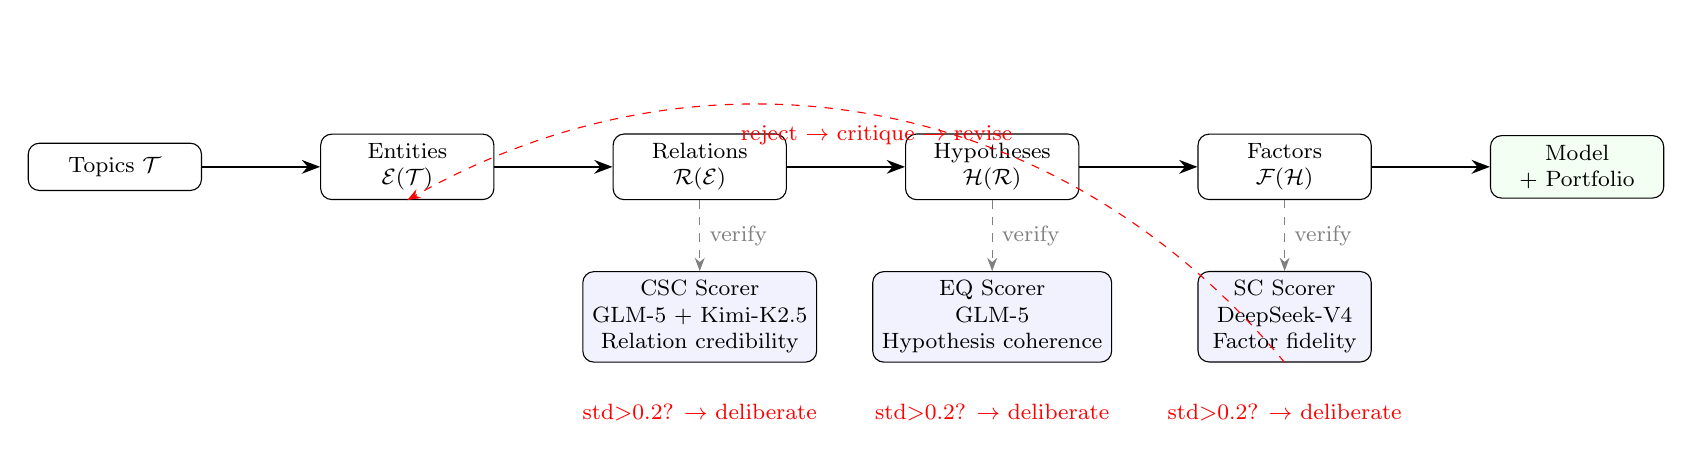
\begin{tikzpicture}[
    node distance=0.5cm,
    stage/.style={rectangle, draw, rounded corners, minimum width=2.2cm, minimum height=0.6cm, align=center, font=\footnotesize},
    scorer/.style={rectangle, draw, rounded corners, fill=blue!5, minimum width=2.2cm, minimum height=0.55cm, align=center, font=\footnotesize},
    arrow/.style={-{Stealth}, thick},
    dasharrow/.style={-{Stealth}, dashed, gray},
]
    % Pipeline stages
    \node[stage] (topic) at (0,0) {Topics $\mathcal{T}$};
    \node[stage, right=1.5cm of topic] (entity) {Entities\\$\mathcal{E}(\mathcal{T})$};
    \node[stage, right=1.5cm of entity] (relation) {Relations\\$\mathcal{R}(\mathcal{E})$};
    \node[stage, right=1.5cm of relation] (hyp) {Hypotheses\\$\mathcal{H}(\mathcal{R})$};
    \node[stage, right=1.5cm of hyp] (factor) {Factors\\$\mathcal{F}(\mathcal{H})$};
    \node[stage, right=1.5cm of factor, fill=green!5] (model) {Model\\+ Portfolio};

    % Arrows between stages
    \draw[arrow] (topic) -- (entity);
    \draw[arrow] (entity) -- (relation);
    \draw[arrow] (relation) -- (hyp);
    \draw[arrow] (hyp) -- (factor);
    \draw[arrow] (factor) -- (model);

    % Scorer agents below
    \node[scorer, below=0.9cm of relation] (csc) {CSC Scorer\\GLM-5 + Kimi-K2.5\\\footnotesize Relation credibility};
    \node[scorer, below=0.9cm of hyp] (eq) {EQ Scorer\\GLM-5\\\footnotesize Hypothesis coherence};
    \node[scorer, below=0.9cm of factor] (sc) {SC Scorer\\DeepSeek-V4\\\footnotesize Factor fidelity};

    % Verification arrows
    \draw[dasharrow] (relation) -- (csc) node[midway, right, font=\footnotesize] {verify};
    \draw[dasharrow] (hyp) -- (eq) node[midway, right, font=\footnotesize] {verify};
    \draw[dasharrow] (factor) -- (sc) node[midway, right, font=\footnotesize] {verify};

    % Deliberation indicators
    \node[below=0.4cm of csc, font=\footnotesize, red] {std$>$0.2? $\rightarrow$ deliberate};
    \node[below=0.4cm of eq, font=\footnotesize, red] {std$>$0.2? $\rightarrow$ deliberate};
    \node[below=0.4cm of sc, font=\footnotesize, red] {std$>$0.2? $\rightarrow$ deliberate};

    % Feedback loop
    \draw[dasharrow, red, bend right=40] (sc.south) to node[below, font=\footnotesize] {reject $\rightarrow$ critique $\rightarrow$ revise} (entity.south);
\end{tikzpicture}
\caption{Topic-to-factor pipeline with stage-wise multi-agent verification. At each semantic transition, independent scorer agents evaluate the intermediate artifact. When scorers disagree (std $>$ 0.2), deliberation is triggered. Rejected artifacts enter the feedback loop for revision.}
\label{fig:pipeline}
\end{figure}

The pipeline transforms user-provided topics into executable factors through four generation stages (Figure~\ref{fig:pipeline}). A Generator LLM ($A_G$, Qwen3.5-Plus) produces entities, relations, hypotheses, and factor expressions in sequence. \textbf{At each transition, independent scorer agents evaluate the artifact before it feeds downstream.} Three scorer types are deployed:

\begin{itemize}
    \item \textbf{CSC Scorer} ($A_{CSC}$): Evaluates relation credibility using two independent LLM instances (GLM-5 and Kimi-K2.5). Assesses existence (does the relation hold?), logical consistency (is it economically sound?), and overall confidence.
    \item \textbf{EQ Scorer} ($A_{EQ}$): Evaluates hypothesis coherence---clarity, economic logic, testability---using GLM-5.
    \item \textbf{SC Scorer} ($A_{SC}$): Evaluates semantic fidelity between factor expressions and source hypotheses---does the formula still track the original rationale? Uses DeepSeek-V4.
\end{itemize}

Each scorer produces a 0--1 quality score. Artifacts survive only if all active gates are satisfied: $\text{CSC} \ge 0.8 \land \text{EQ} \ge 0.75 \land \text{SC} \ge 0.8$. The \texttt{no\_kg} baseline removes all gates; ablation variants (\texttt{no\_csc}, \texttt{no\_eq}, \texttt{no\_sc}) remove one gate at a time.

\subsection{Why Multiple Scorers? The Case Against Single-Scorer Verification}

A natural question is whether a single scorer per stage suffices. We evaluated a single LLM scorer against human judgment on 51 relations~\footnote{Human evaluation: one evaluator scored each relation holistically, then re-scored using a structured rubric (existence/logic/evidence sub-dimensions).}. The overall Spearman correlation of $r{=}0.61$ is moderate, but this masks a critical failure pattern: in the medium-quality range (LLM fused scores 0.5--0.8), the correlation collapses to $r{=}0.02$---essentially random. These borderline artifacts are precisely where verification matters most for downstream factor quality, because they are the ones that would be kept or discarded based on small threshold differences.

Using multiple scorers helps: inter-scorer agreement on the full Layer-3 dataset (809 relations, GLM-5 vs.\ Kimi-K2.5) is $r{=}0.77$, with 21.5\% exhibiting significant disagreement (std $>$ 0.2). Two scorers disagree most on borderline artifacts---exactly where a single scorer is unreliable. But multiple scorers introduce a new problem: how to fuse their judgments.

\subsection{Deliberative Consensus: When Voting Fails}

\begin{algorithm}[t]
\caption{Deliberative Consensus Protocol}
\label{alg:deliberation}
\KwIn{Artifact $a$, scores $\{s_m\}$, thresholds $\theta_d{=}0.2$, $\theta_c{=}0.1$, max rounds $R_{\max}{=}3$}
\KwOut{Final scores, convergence status}

$\sigma_0 \leftarrow \text{StdDev}(\{s_m\})$\;
\If{$\sigma_0 \leq \theta_d$}{\Return{($\{s_m\}$, \texttt{CONSENSUS})}}
$r \leftarrow 1$\;

\While{$r \leq R_{\max}$}{
    \ForEach{scorer $m$}{
        prompt$_m \leftarrow$ BuildPrompt($a$, $\{s_m\}$, peer scores + reasoning)\;
        $(s'_m, \text{reasoning}_m) \leftarrow$ LLM($m$, prompt$_m$)\;
    }
    $\sigma_r \leftarrow \text{StdDev}(\{s'_m\})$\;
    \If{$\sigma_r \leq \theta_c$}{\Return{($\{s'_m\}$, \texttt{CONSENSUS})}}
    $r \leftarrow r + 1$\;
}
\Return{($\{s'_m\}$, \texttt{CONTROVERSIAL})}\;
\end{algorithm}

The default approach to fusing multiple scorers---simple averaging---has a severe failure mode. Our 5-model heterogeneity study (30 relations scored independently by Qwen3.7-Max, GLM-5.2, Kimi-K2.7, MiniMax-M3, and DeepSeek-V4-Pro) reveals two critical findings:

\begin{figure}[t]
\centering
\includegraphics[width=0.75\columnwidth]{figures/fig_heterogeneity_heatmap.pdf}
\caption{Pairwise Spearman correlations of 5 scorer models. Qwen and Kimi are highly correlated with each other ($r{=}0.91$) and with human judgment ($r{=}0.89$, $0.91$). GLM and DeepSeek are negatively correlated with the best models. More scorers do not mean better consensus.}
\label{fig:heterogeneity}
\end{figure}

\textbf{First, scorer quality varies dramatically} (Figure~\ref{fig:heterogeneity}): Qwen ($r{=}0.89$ with human) and Kimi ($r{=}0.91$) are strong; GLM ($r{=}-0.15$) and DeepSeek ($r{=}-0.08$) are essentially uncorrelated with human judgment. \textbf{Second, adding poor scorers degrades consensus}: the best single model (Kimi, $r{=}0.91$) outperforms the 3-model ($r{=}0.85$) and 5-model ($r{=}0.81$) averages.

Most critically: on the 13 relations where Qwen and Kimi genuinely disagree (std $>$ 0.05), \textbf{simple averaging degrades accuracy in 62\% of cases (8/13; across all 6 model pairs: 55\%, bootstrap 95\% CI 46--63\%, $n{=}130$)}. Consider ``CAPM $\rightarrow$ Short-Term Reversal Factor'' (human score 0.80): Qwen assigns 0.20 (incorrectly rejecting it) while Kimi assigns 0.90 (correctly accepting). Averaging yields 0.55---worse than Kimi alone---because Qwen's error receives equal weight.

This failure mode motivates the deliberative consensus protocol (Algorithm~\ref{alg:deliberation}). When disagreement exceeds $\theta_d{=}0.2$, each scorer receives a deliberation prompt containing: the artifact, their own prior score and reasoning, and all peer scores and reasoning. Scorers independently re-evaluate---they may maintain, revise, or partially adjust, but must explain their reasoning in response to peer critiques. The loop continues until std drops below $\theta_c{=}0.1$ or a maximum of 3 rounds.

\subsection{Agentic Feedback Loop}

Artifacts that fail verification (fused score $<$ 0.6) are not discarded. The scorer's structured critique is routed back to the Generator, which revises and re-submits (max 3 rounds). This transforms one-pass generation into a closed-loop self-correction harness.

% ======================================================================
\section{Case Study: Factor Discovery Deployment}
% ======================================================================

The architecture is deployed for quantitative finance factor discovery on Chinese A-shares. Four user-provided topics (financial metrics, economic theories, factor patterns, market institutions) seed the pipeline. The Generator produces $\sim$800 candidate relations, of which $\sim$500 survive CSC verification. These feed hypothesis and factor generation, with EQ and SC verification at each stage. The final selector retains factors passing all three gates.

All experiments use a shared feature store with manifest-driven discovery. The downstream model is LightGBM with fixed hyperparameters across all runs. Each configuration is evaluated via TopK-Dropout portfolio strategy (top 50 stocks, 5 dropped daily, 10 bps transaction cost). Training: 2022--2023; out-of-sample: 2024H2--2025 (368 trading days). Primary endpoints: ARR, IR, MDD. Two evaluation axes: cross-market (full vs.\ no\_kg on CSI300/500/800/1000) and agent ablation (removing one scorer at a time on CSI800).

The complete agent harness ($\sim$2,000 lines of Python: protocol, deliberation, feedback loop, harness) is released as open-source at \url{https://github.com/yangguang760/kg-agent-quant}.

% ======================================================================
\section{Results}
% ======================================================================

\subsection{Pipeline Effectiveness: Cross-Market Performance}

Table~\ref{tab:cross} reports portfolio metrics. The full multi-agent verification configuration outperforms the no-verification baseline (Alpha158 factors only, no KG pipeline) in three of four markets. CSI800 shows the largest absolute gain (ARR +0.091), CSI1000 (+0.087) and CSI500 (+0.099) also benefit. CSI300 is the exception---full underperforms no\_kg---establishing a clear boundary condition.

\begin{table}[t]
\caption{Cross-market portfolio metrics. Full = all verification gates active. no\_kg = Alpha158 baseline (no KG pipeline). Bold: higher value within each universe.}
\label{tab:cross}
\centering
\begin{tabular}{l l r r r r}
\toprule
Market & Config & IC & ARR & IR & MDD \\
\midrule
CSI300 & full & 0.001 & $-$0.047 & $-$0.70 & $-$0.11 \\
CSI300 & no\_kg & 0.011 & \textbf{0.046} & \textbf{0.58} & \textbf{$-$0.09} \\
CSI500 & full & 0.002 & \textbf{0.137} & \textbf{1.09} & \textbf{$-$0.08} \\
CSI500 & no\_kg & 0.004 & 0.039 & 0.35 & $-$0.11 \\
CSI800 & full & 0.010 & \textbf{0.209} & \textbf{1.77} & \textbf{$-$0.06} \\
CSI800 & no\_kg & 0.009 & 0.118 & 1.17 & $-$0.07 \\
CSI1000 & full & 0.014 & \textbf{0.242} & \textbf{1.41} & \textbf{$-$0.11} \\
CSI1000 & no\_kg & 0.020 & 0.155 & 1.07 & $-$0.10 \\
\bottomrule
\end{tabular}
\end{table}

Agent ablation on CSI800 (Table~\ref{tab:ablation}) confirms that \textbf{each scorer contributes independently}: removing any gate degrades performance. EQ removal causes the largest decline ($-$39\% ARR), followed by SC ($-$29\%) and CSC ($-$15\%). The ordering reflects the training horizon: with 2 years of training data, hypothesis coherence becomes the rate-limiting verification gate. Column counts corroborate: SC is the most permissive single gate (287 columns when removed vs.\ 111 with all gates), indicating that many borderline factor expressions are correctly excluded by the SC check.

\begin{table}[t]
\caption{Agent ablation on CSI800. Each scorer removed independently. Column count reflects selector-level impact of each gate.}
\label{tab:ablation}
\centering
\begin{tabular}{l r r r r r}
\toprule
Config & Cols & IC & ARR & IR & MDD \\
\midrule
full (all scorers) & 111 & 0.010 & 0.209 & 1.77 & $-$0.06 \\
no\_csc & 154 & 0.007 & 0.178 & 1.52 & $-$0.05 \\
no\_eq  & 145 & 0.006 & 0.127 & 1.00 & $-$0.08 \\
no\_sc  & 287 & 0.004 & 0.148 & 1.19 & $-$0.07 \\
\bottomrule
\end{tabular}
\end{table}

\subsection{Why Voting Fails, and How Deliberation Fixes It}

The heterogeneity study (Section 2.2, Figure~\ref{fig:heterogeneity}) established that simple multi-scorer averaging fails on disagreement cases. Table~\ref{tab:deliberation} reports the result of applying deliberative consensus instead, evaluated on 19 relations with genuine inter-scorer disagreement across two independent scorer configurations.

\begin{table}[t]
\caption{Deliberation results across two scorer configurations. Homo: 2$\times$DeepSeek-V4-Pro. Hetero: Qwen3.7-Max vs.\ Kimi-K2.7.}
\label{tab:deliberation}
\centering
\begin{tabular}{l r r}
\toprule
Metric & Homo (DS$\times$2, n=10) & Hetero (Qwen+Kimi, n=9) \\
\midrule
Convergence rate (std$<$0.10) & 80\% & 89\% \\
Mean primary std & 0.203 & 0.161 \\
Mean final std & 0.048 & 0.068 \\
Mean std reduction & 0.155 & 0.093 \\
Mean primary human error & 0.243 & 0.111 \\
Mean final human error & 0.238 & 0.092 \\
Human error reduction & $-$2\% & $-$17\% \\
\bottomrule
\end{tabular}
\end{table}

\begin{figure}[t]
\centering
\includegraphics[width=0.92\columnwidth]{figures/fig_deliberation_comparison.pdf}
\caption{Deliberation reduces scorer disagreement (left) and human error (right) in both homogeneous and heterogeneous settings. Heterogeneous deliberation starts from a better baseline (lower initial human error) because Qwen and Kimi are individually more accurate scorers.}
\label{fig:deliberation}
\end{figure}

Three patterns emerge. First, \textbf{deliberation robustly resolves disagreement} (Figure~\ref{fig:deliberation}): 80--89\% of relations converge, with std reductions of 0.09--0.16. Scorers do not simply repeat initial judgments---the mean score shift is 0.19 (homo) and 0.05 (hetero). Second, \textbf{heterogeneous deliberation starts from a better baseline} (human error 0.111 vs.\ 0.243 for homo) because Qwen and Kimi are individually more accurate scorers, and further reduces error by 17\%. Third, \textbf{deliberation is not infallible}: in 4/10 (homo) and 5/9 (hetero) cases, post-deliberation consensus moved farther from human judgment---the ``confident incorrect majority'' problem, where a correct dissenter is persuaded toward an incorrect consensus. This motivates our architecture's preservation of the \texttt{CONTROVERSIAL} flag for human review.

\subsection{Human Validation and Feedback Loop}

Human validation (51 relations) confirms that LLM scorer quality approaches human-level reliability: Spearman $r{=}0.61$ between LLM and human, compared to $r{=}0.57$ between holistic and rubric-based human scoring (intra-rater). Two systematic LLM biases were identified: overrating creative-but-weak relations and underrating tautological-but-correct ones.

The agentic feedback loop was evaluated on 15 rejected artifacts. 53\% (8/15) pass re-verification after revision (mean score improvement +0.13), with major content revisions being most effective. Full details on threshold sensitivity (19 sweep experiments), human evaluation methodology, feedback loop analysis, and deployment cost are provided in the Appendix.

% ======================================================================
\section{Discussion: Lessons Learned}
% ======================================================================

\subsection{Replace Voting with Deliberation When Scorers Disagree}

The most actionable finding is that \textbf{simple multi-model voting reliably fails on the cases where it matters most}. When scorers disagree---which happens on 21.5\% of artifacts and is concentrated in the borderline quality range where single-scorer reliability collapses---equal-weight averaging degrades accuracy in 55\% of disagreement cases (bootstrap 95\% CI: 46--63\%, $n{=}130$). The fix is deliberation: let scorers exchange reasoning rather than blindly averaging. Our deliberation experiments (19 relations across two scorer configurations) confirm that structured debate converges 80--89\% of disagreements, with the largest improvements on the most disputed artifacts.

\subsection{Scorer Quality Dominates Scorer Quantity}

Adding more scorers improves verification only when the added scorers are individually competent and genuinely complementary. Our heterogeneity study shows that the best 2-model consensus ($r{=}0.90$) outperforms the 5-model consensus ($r{=}0.81$) because three of five models have near-zero correlation with human judgment. For practitioners, the practical guideline is: evaluate candidate scorer models against a small set of human-labeled examples (30--50 artifacts, $\sim$2 hours of annotation effort), select the top 2--3 that are both individually accurate and mutually complementary (pairwise $r$ below 0.95 to avoid redundancy), and deploy them with deliberation rather than voting.

\subsection{Boundaries and Limitations}

The cross-market results establish clear boundary conditions: the pipeline benefits CSI800, CSI1000, and CSI500, but not CSI300. CSI300's failure is informative: as a pure large-cap index (top 300 stocks by market cap), it represents the most efficient segment of the A-share market, where factor-based alpha is hardest to extract. CSI800 and CSI1000, which include mid- and small-cap constituents with lower analyst coverage and higher dispersion, provide richer soil for KG-generated factors. This pattern---stronger factor efficacy in broader, less efficient universes---is consistent with the factor investing literature. For practitioners, the lesson is that multi-agent verification adds the most value in less efficient market segments where the generator produces a wider quality spectrum of candidate factors. Deployment decisions should be informed by per-market validation. The evidence is for Chinese equities over 2022--2025; generalization requires further validation. The human evaluation uses a single evaluator with two methods (intra-rater); multi-evaluator inter-rater studies would strengthen scorer quality claims.

% ======================================================================
\section{Related Work}
% ======================================================================

Multi-agent LLM verification uses independent agents to reduce self-verification bias~\cite{wang2025masllm,ghafarollahi2024sciagents,mao2025blueprint2code}. SC-MoA demonstrates that reading reasoning traces recovers correct answers even under unanimous wrong votes; A-HMAD introduces heterogeneous debate with learned consensus weighting; AI Council reveals that homogeneous evaluators artificially converge; Aegean reframes consensus as a distributed systems problem. Our work differs by (i) applying verification at \emph{intermediate} pipeline stages rather than only final outputs, (ii) empirically demonstrating why simple averaging fails in a real deployment, and (iii) providing full-scale deliberation evidence integrated with staged gates and feedback loops.

Google's A2A protocol standardizes agent discovery; MCP standardizes tool connectivity; LangGraph/CrewAI/AutoGen provide orchestration patterns. Our inter-agent protocol adopts A2A-inspired design while specializing for verification workflows.

Automated factor discovery has progressed from evolutionary search~\cite{kakushadze2016101} to LLM-assisted systems~\cite{wang2024alphagpt,tang2025alphaagent,shi2025alphaforge}. Knowledge-guided approaches constrain generation with domain structure~\cite{guo2022quant40,lin2026factorengine}. Our contribution treats the knowledge structure as an agent-constructed artifact requiring verification, placing it at the intersection of multi-agent verification and factor discovery.

% ======================================================================
\section{Conclusion}
% ======================================================================

We presented a multi-agent verification architecture for topic-to-factor LLM pipelines, with a deliberative consensus protocol that replaces simple averaging when scorers disagree. Full-scale deployment on Chinese equity markets demonstrates pipeline effectiveness in three of four universes, and a 19-relation deliberation experiment across two scorer configurations confirms that structured debate converges 80--89\% of disagreements. The key practical lesson is that scorer quality and deliberation design matter more than the number of scorers. We release the complete system as open-source software.

% ======================================================================
% Bibliography
% ======================================================================

\bibliographystyle{ACM-Reference-Format}
\bibliography{../.paper-output/references}

% ======================================================================
% APPENDIX
% ======================================================================
\clearpage
\appendix
\section{Appendix}

\subsection{Threshold Sensitivity}

\begin{table}[h]
\caption{Threshold sensitivity on CSI800. Each gate varied independently; others held at defaults (CSC=0.8, EQ=0.75, SC=0.8). Bold: best ARR.}
\label{tab:threshold_appendix}
\centering
\begin{tabular}{l r r r r}
\toprule
Gate \& Threshold & Cols & IC & ARR & IR \\
\midrule
\multicolumn{5}{l}{\textbf{CSC sweep}} \\
CSC=0.4 & 154 & $-$0.004 & 0.080 & 0.75 \\
CSC=0.6 & 153 & $-$0.002 & 0.165 & 1.46 \\
CSC=0.8 & 111 & 0.001 & \textbf{0.181} & 1.69 \\
CSC=0.9 & 37 & $-$0.005 & 0.071 & 0.70 \\
\midrule
\multicolumn{5}{l}{\textbf{EQ sweep}} \\
EQ=0.4--0.7 & 145 & 0.000 & 0.136 & 1.38 \\
EQ=0.75 & 111 & 0.001 & \textbf{0.181} & 1.69 \\
EQ=0.8 & 79 & $-$0.001 & 0.130 & 1.31 \\
EQ=0.9 & 3 & $-$0.002 & 0.168 & 1.52 \\
\midrule
\multicolumn{5}{l}{\textbf{SC sweep}} \\
SC=0.4--0.5 & 287 & $-$0.008 & 0.131 & 1.60 \\
SC=0.6 & 253 & 0.002 & 0.121 & 1.46 \\
SC=0.7 & 181 & $-$0.001 & \textbf{0.189} & 1.81 \\
SC=0.8 & 111 & 0.001 & 0.181 & 1.69 \\
SC=0.9 & 38 & 0.003 & 0.152 & 1.32 \\
\bottomrule
\end{tabular}
\end{table}

The SC=0.7--0.8 borderline zone (70 factors) contains mixed-quality artifacts that a fixed threshold cannot distinguish. Deliberation provides per-artifact discrimination in this zone.

\begin{figure}[h]
\centering
\includegraphics[width=0.7\columnwidth]{figures/fig_threshold_sensitivity.pdf}
\caption{SC threshold sweep. ARR peaks at SC=0.7 (0.189). The borderline zone (shaded) contains 70 mixed-quality factors.}
\label{fig:threshold_appendix}
\end{figure}

\subsection{Human Validation}

Human evaluation used 51 relations stratified by LLM fused score (17 each from high/medium/low). The evaluator scored holistically (0--1), then re-scored using structured rubric (existence/logic/evidence sub-dimensions averaged).

\begin{table}[h]
\caption{Human-LLM and intra-rater agreement (n=51).}
\label{tab:human_appendix}
\centering
\begin{tabular}{l r r}
\toprule
Metric & H1-LLM & H1-H2 (intra-rater) \\
\midrule
Spearman $r$ (overall) & 0.61 & 0.57 \\
Spearman $r$ (LLM $\ge$0.8) & 0.49 & 0.53 \\
Spearman $r$ (LLM 0.5--0.8) & 0.02 & 0.42 \\
Spearman $r$ (LLM $<$0.5) & 0.66 & 0.57 \\
\bottomrule
\end{tabular}
\end{table}

Two systematic LLM biases: (1) overrating creative-but-weak relations (e.g., Fama-French $\rightarrow$ Dividend Yield: LLM 0.78 vs.\ human 0.35), (2) underrating tautological-but-correct relations (e.g., Low PB $\rightarrow$ Value Style Market: LLM 0.48 vs.\ human 0.80).

\subsection{Feedback Loop and Cost}

\begin{table}[h]
\caption{Agentic feedback loop (15 rejected relations).}
\label{tab:feedback_appendix}
\centering
\begin{tabular}{l r}
\toprule
Metric & Value \\
\midrule
Score improved after revision & 7/15 (47\%) \\
Passed threshold ($\ge$0.6) after revision & 8/15 (53\%) \\
Content meaningfully changed & 5/15 (33\%) \\
Mean score before / after & 0.39 / 0.52 (+0.13) \\
\bottomrule
\end{tabular}
\end{table}

\textbf{Deployment cost:} Full pipeline requires $\sim$3,000 API calls per 1,000 candidate relations (3$\times$ single-pass). 78.5\% of artifacts incur only 2$\times$ primary scoring; deliberation (21.5\% controversy) and feedback (29.3\% rejection) are concentrated on borderline cases. At current API pricing, $\sim$\$2.50--\$5.00 per 1,000 relations.

\subsection{Agent Configuration}

\begin{table}[h]
\caption{LLM configuration used in deployment.}
\centering
\begin{tabular}{l l l l}
\toprule
Agent Role & Provider & Model & $\tau$ \\
\midrule
Generator & Alibaba & Qwen3.5-Plus & 0.7 \\
CSC Scorer (1) & Zhipu & GLM-5 & 0.3 \\
CSC Scorer (2) & Moonshot & Kimi-K2.5 & 0.3 \\
EQ Scorer & Zhipu & GLM-5 & 0.3 \\
SC Scorer & DeepSeek & DeepSeek-V4 & 0.3 \\
\bottomrule
\end{tabular}
\end{table}

\end{document}
